\chapter[Algoritmos]{Algoritmos}
\label{cap:formato}

Este capítulo apresenta os algoritmos utilizados nesse trabalho e faz uma análise a discussão sobre a viabilidade/aplicabilidade de cada um deles. 

A entrada de dados foi padronizada para : Os n itens da loja serão fornecidos em um arquivo texto que contêm na primeira linha W (capacidade da mochila), na segunda linha n (número de itens) e nas linhas seguintes os itens, cada
um em uma linha (contendo o peso seguido do valor). Os valores devem ser números inteiros.

Enquanto a saida seria: 

a) um arquivo texto contendo, nesta ordem:
\begin{itemize}
\item para cada item escolhido para a solução, o número do item, seu peso e seu valor (uma
linha por item)
\item uma linha contendo o somatório dos pesos dos itens escolhidos
\item  uma linha contendo o somatório dos valores dos itens. 
\end{itemize}
b) a impressão na tela do tempo total de execução do programa.

Devido a essa padronização, de entradas e saídas, parte dos programas se repete.
\section{Algoritmo Guloso}
\label{sec:preTextual}
 O algoritmo guloso é geralmente descrito como um algoritmo \textit{míope}, pois toma decições baseado nas melhores esolhas locais, isso é, nunca olha os resultados dessa escolhas futuramente. Muitas poucas vezes os algoritmos gulosos apresentam resoluções ótimas, porém apresentam resoluções perto das ótimas em uma quantidade razoável de vezes. 
 
\subsection{Análise do Algoritmo}
 A Figura 1 representa a esquematização do algoritmo, onde se aplica cria o TAD (tipo abstrato de dado) Objeto, que é composto de um peso e um valor. Após a criação de um vetor de Objetos, se organiza esse vetor e aplica o vetor ordenado na função Guloso, que retorna o resultado.

\begin{figure}[htb!]
    \centering
    \caption{Algoritmo Guloso}
    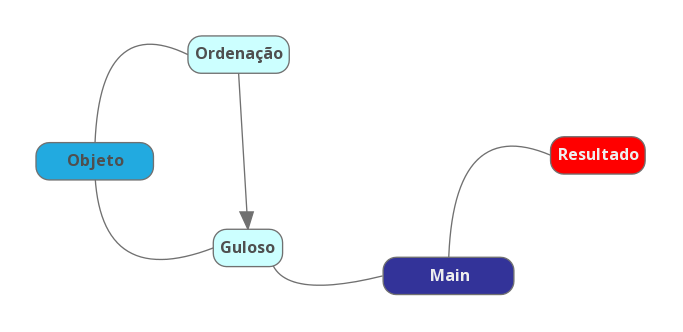
\includegraphics[keepaspectratio=true,scale=0.8]
    	{img/GULOSO.png}
    \label{fig:elementos}
\end{figure}


%O nome do capítulo, apêndice e anexo deve ser sempre em maíuscula e, das seções, em com a letra de cada palavra em maiúscula (exceto preposições e artigos).

\section{Algoritmo de Tentativa e Erro}
\label{sec:textual}







\subsection{Exemplo de Seção de Nível 2}
\subsubsection{Exemplo de Seção de Nível 3}
\subsubsubsection{Exemplo de Seção de Nível 4}

Segundo a \cite{abntTxtAcad2011}, a numeração dos elementos textuais, quando utilizado apenas a frente da folha, deverá ser apresentada no canto direito superior. Quando, no TCC, utiliza-se a frente e o verso da folha, a frente deverá possuir a numeração no canto direito superior e, o verso, no canto esquerdo superior.

\begin{figure}[htb!]
    \centering
    \caption{Desenho feito por Daniel Hasan Dalip.}
    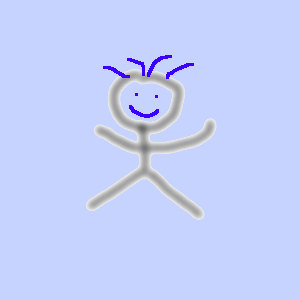
\includegraphics[keepaspectratio=true,scale=0.62]
    	{img/desenho.png}
    \fonte{Daniel Hasan Dalip.}
    \label{fig:desenhoAutor}
\end{figure}

Seguindo as normas  \cite{ibge1993,abntTxtAcad2011}, conforme apresentado nas Figuras~\ref{fig:elementos} e \ref{fig:desenhoAutor}, cada ilustração deve possuir o seu título na parte superior e a fonte de onde foi retirada esta figura na parte inferior. É importante notar que é obrigatório colocar a fonte consultada, mesmo que esta seja o próprio autor. As tabelas devem ser apresentadas conforme a Tabela~\ref{tab:exemploTabela}. Caso queira mais exemplos de tabelas, 
conferir o padrão~\citeonline{ibge1993}. 

\begin{table}[]
\centering
\caption{Exemplo de tabela}
\label{tab:exemploTabela}
\begin{tabular}{lll}
\toprule
Coluna 1                                              & Coluna 2            & Coluna 3 \\ \midrule
21		                                              & 21            		& 212 \\ 
11		                                              & 23            		& 32 \\ 
10		                                              & 11		            & 32 \\ \bottomrule
\end{tabular}
\fonte{Produzido por Daniel H. Dalip e Glívia Angélica.}
\end{table}

As equações podem ser feitas ao longo do texto, por exemplo: $area = \frac{base \times altura}{2}$ ou apresentadas no ambiente \textit{equation}, como na Equação~\ref{eq:testeEquacao}.
\begin{equation}
	area = \frac{base \times altura}{2}
    \label{eq:testeEquacao}
\end{equation}

Finalmente, os textos possuem citações bibliográficas. A padronização das citações são apresentadas por~\citeonline{abntCitacoes2002}. A citação deve ser feita da seguinte forma: caso o nome do autor faça parte do texto, deve-se colocar entre parênteses apenas o ano por exemplo: \citeonline{brin1998anatomy} apresentaram o algoritmo PageRank. Caso contrário, o nome do autor ficará entre parênteses, por exemplo: neste método foi utilizado o algoritmo Page Rank~\cite{brin1998anatomy,abntCitacoes2002}.


\section{Elementos Pós-textuais}
\label{sec:posTextual}

Os elementos pós-textuais são compostos das referências Bibliográficas, Apêndice e Anexos. A ABNT não estabelece um padrão o título dessas seções. No presente documento, seguindo o template do ABNTex2, utilizou-se a fonte \textit{Latin Modern Sans} tamanho 24pt. Deverá haver numeração das páginas. Lembre-se: apêndice são materiais produzidos pelo autor do TCC enquanto anexo são materiais produzidos por outros autores. 
As normas de referencias estão disponíveis em~\cite{abntCitacoes2002}\footnote{Neste site é possível verificar alguns exemplos: \url{http://www.leffa.pro.br/textos/abnt.htm}}.